\documentclass[]{beamer}\usepackage[]{graphicx}\usepackage[]{color}
% maxwidth is the original width if it is less than linewidth
% otherwise use linewidth (to make sure the graphics do not exceed the margin)
\makeatletter
\def\maxwidth{ %
  \ifdim\Gin@nat@width>\linewidth
    \linewidth
  \else
    \Gin@nat@width
  \fi
}
\makeatother

\definecolor{fgcolor}{rgb}{0.345, 0.345, 0.345}
\newcommand{\hlnum}[1]{\textcolor[rgb]{0.686,0.059,0.569}{#1}}%
\newcommand{\hlstr}[1]{\textcolor[rgb]{0.192,0.494,0.8}{#1}}%
\newcommand{\hlcom}[1]{\textcolor[rgb]{0.678,0.584,0.686}{\textit{#1}}}%
\newcommand{\hlopt}[1]{\textcolor[rgb]{0,0,0}{#1}}%
\newcommand{\hlstd}[1]{\textcolor[rgb]{0.345,0.345,0.345}{#1}}%
\newcommand{\hlkwa}[1]{\textcolor[rgb]{0.161,0.373,0.58}{\textbf{#1}}}%
\newcommand{\hlkwb}[1]{\textcolor[rgb]{0.69,0.353,0.396}{#1}}%
\newcommand{\hlkwc}[1]{\textcolor[rgb]{0.333,0.667,0.333}{#1}}%
\newcommand{\hlkwd}[1]{\textcolor[rgb]{0.737,0.353,0.396}{\textbf{#1}}}%
\let\hlipl\hlkwb

\usepackage{framed}
\makeatletter
\newenvironment{kframe}{%
 \def\at@end@of@kframe{}%
 \ifinner\ifhmode%
  \def\at@end@of@kframe{\end{minipage}}%
  \begin{minipage}{\columnwidth}%
 \fi\fi%
 \def\FrameCommand##1{\hskip\@totalleftmargin \hskip-\fboxsep
 \colorbox{shadecolor}{##1}\hskip-\fboxsep
     % There is no \\@totalrightmargin, so:
     \hskip-\linewidth \hskip-\@totalleftmargin \hskip\columnwidth}%
 \MakeFramed {\advance\hsize-\width
   \@totalleftmargin\z@ \linewidth\hsize
   \@setminipage}}%
 {\par\unskip\endMakeFramed%
 \at@end@of@kframe}
\makeatother

\definecolor{shadecolor}{rgb}{.97, .97, .97}
\definecolor{messagecolor}{rgb}{0, 0, 0}
\definecolor{warningcolor}{rgb}{1, 0, 1}
\definecolor{errorcolor}{rgb}{1, 0, 0}
\newenvironment{knitrout}{}{} % an empty environment to be redefined in TeX

\usepackage{alltt}
%% \documentclass[notes]{beamer} %% include notes.

\newcommand{\Slang}{\texttt{S} }
\newcommand{\R}{\texttt{R} }
\newcommand{\Rfunction}[1]{{\texttt{#1}}}
\newcommand{\Robject}[1]{{\texttt{#1}}}
\newcommand{\Rpackage}[1]{{\mbox{\normalfont\textsf{#1}}}}

\definecolor{Red}{rgb}{0.7,0,0}
\definecolor{Blue}{rgb}{0,0,0.8}
\usepackage{fancyvrb}
\usepackage{hyperref,verbatim}
\hypersetup{%
  pdfusetitle,
  bookmarks = {true},
  bookmarksnumbered = {true},
  bookmarksopen = {true},
  bookmarksopenlevel = 2,
  unicode = {true},
  breaklinks = {false},
  hyperindex = {true},
  colorlinks = {true},
  linktocpage = {true},
  plainpages = {false},
  linkcolor = {Blue},
  citecolor = {Blue},
  urlcolor = {Red},
  pdfstartview = {Fit},
  pdfpagemode = {UseOutlines},
  pdfview = {XYZ null null null}
}


%% Lecture notes have been made using the Beamer class for LaTeX.
%% http://latex-beamer.sourceforge.net/ 
%% 
%% You will also need textpos.sty, which comes via:
%% http://www.ctan.org/tex-archive/macros/latex/contrib/textpos/
%% 
%% There is an extra makefile that will help with creating versions of
%% the lecture notes either for the lecturer:
%% 
%% make rpc.pdf
%% 
%% or the student (4-up, A4 paper):
%% 
%% make h.pdf

%% If the 'Outline' slides are empty, try 'pdflatex rpc' after 'make
%% rpc.pdf' and they should appear.  (Any hints on how to fix this in
%% the Makefile?)

%% This file also includes some notes, which are included in the
%% output if you pass the [notes] option to the beamer documentclass,
%% see above.  (Look for \note{...} in slides below.}

%% Default will be false for this ifhandouts.  Set handouts to true
%% and then you will get 4up handouts suitable for a4paper.
\usepackage{ifthen}
\providecommand*{\handouts}{false}

%% lecs: 
%% \includeonlylecture{sat}


%% Following is useful for getting 4-up output directly to A4 pdf.
\ifthenelse{\equal{\handouts}{true}}
{\usepackage{pgfpages}
  \pgfpagesuselayout{4 on 1}[a4paper,landscape]}
{}

\usepackage{bm}                 %Bold math allows Greeksymbols in bold.


%% Listings package is used for including R commands etc.
\usepackage{listings}

\lstset{commentstyle=\color{red},keywordstyle=\color{black},
  showstringspaces=false}
\lstnewenvironment{rc}[1][]{\lstset{language=R}}{}
%% \newenvironment{rc} {\begin{alltt}\small} {\end{alltt}}

\newcommand{\adv}{{\tiny (Advanced)}}
\newcommand{\ri}[1]{\lstinline{#1}}  %% Short for 'R inline'

\lstnewenvironment{rc.out}[1][]{\lstset{language=R,%%
    morecomment=[is]{/*}{*/},%
    moredelim=[is][\itshape]{(-}{-)},frame=single}}{}

%% \usepackage{emaxima}
\usepackage[overlay]{textpos}   %For using textblock

\setlength{\TPHorizModule}{10mm}
\setlength{\TPVertModule}{\TPHorizModule}
\newcommand{\ds}{\vspace*{5mm}}
\newcommand{\xstar}{\ensuremath{x^\ast}}

\newcommand{\vmu}{{\bm{\mu}}\xspace}

%% \usepackage{theapa}
\usepackage{amsmath,graphicx}
%% \usepackage{multimedia}         %%Need for movies.

\newcommand{\smallref}[1]{{\small #1}}
%% \newcommand{\mybox}[1]{\fbox{#1}}x

%% \graphicspath{{../talk_figs/}{/home/anotherpath/}}
\graphicspath{{figs/}}

\setlength{\TPHorizModule}{10mm}
\setlength{\TPVertModule}{10mm}

\newcommand{\colhalf}{\column{0.49\textwidth}}

\author{
  Stephen Eglen
  Laurent Gatto
  %% \footnote{\url{lg390@cam.ac.uk}}\footnote{\url{http://proteome.sysbiol.cam.ac.uk/lgatto/teaching/spr.html}}\\ 
}
\date{\today}


\mode<presentation>
{
  \setbeamersize{text margin left=0.25cm}
  \setbeamersize{text margin right=0.25cm}

  \beamertemplatedotitem

  \beamertemplateheadempty %% Remove headline (at top of frame)
  %% \beamertemplatefootempty %% Remove headline (at top of frame)
  \beamertemplatefootpagenumber %% pagenumber only in footer.
  %% Remove navigation icons.
  \beamertemplatenavigationsymbolsempty
  %% Show start of every lecture. Not available in article.
  %% \AtBeginLecture{\begin{frame}{\Large Lecture \insertlecture}\end{frame}}
}

\mode<article>
{
  \usepackage{fullpage}
  \usepackage{pgf}
  \usepackage{hyperref}
  %% \setjobnamebeamerversion{aa}
}

%% This is run at the start of every section.
\AtBeginSection[] % Do nothing for \section*
{
  \begin{frame}<beamer>
    \frametitle{Outline}
    \tableofcontents[currentsection]
    %% \frametitle{currentsection}
  \end{frame}
}

\title{Scientific Programming with \R}
\IfFileExists{upquote.sty}{\usepackage{upquote}}{}
\begin{document}

\lstset{language=R}
%% Switch off title page.
%% \begin{frame}

\mode<article>
{
  \date{\today}
  \maketitle

  These are the lecture notes for the programming course.
}


\mode<presentation>
{
  \date{\today}
  \maketitle
}



\lecture{Reproducible research}{rr}


\begin{frame}
  \frametitle{Literate Programming}

  From the web page describing his book /Literate Programming/, Donald E
  Knuth writes:

  "Literate programming is a methodology that combines a programming
  language with a documentation language, thereby making programs more
  robust, more portable, more easily maintained, and arguably more fun
  to write than programs that are written only in a high-level
  language. The main idea is to treat a program as a piece of
  literature, addressed to human beings rather than to a computer. The
  program is also viewed as a hypertext document, rather like the World
  Wide Web. (Indeed, I used the word WEB for this purpose long before
  CERN grabbed it!) ..."

  \bigskip

  \url{http://www-cs-faculty.stanford.edu/~uno/lp.html}

\end{frame}


\begin{frame}[fragile]
  \frametitle{Tangling and Weaving}

  CWEB: system for documenting C, C++, Java:

\begin{verbatim}
CTANGLE
      converts a source file foo.w to a
      compilable program file foo.c; 
CWEAVE
      converts a source file foo.w to a
      prettily-printable and 
      cross-indexed document file foo.tex. 
\end{verbatim}

\end{frame}


\begin{frame}
  \frametitle{Tangling and weaving}

  \centering 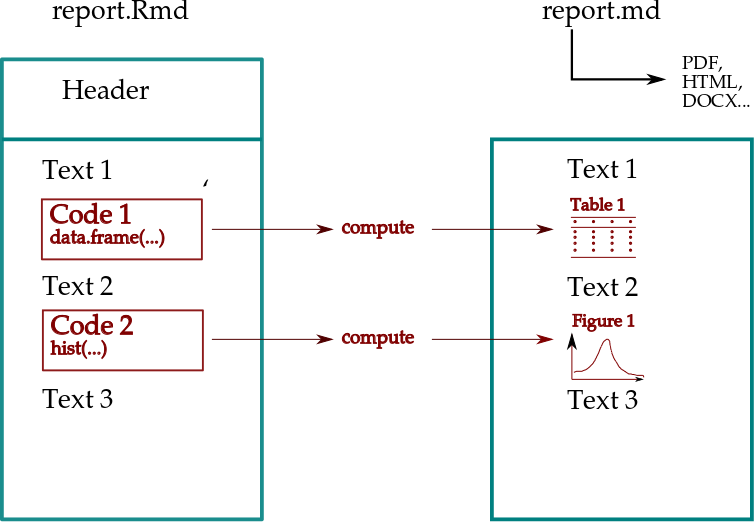
\includegraphics[width=10cm]{rmd-to-md.png}
  
\end{frame}

\begin{frame}


  \frametitle{What is reproducible research (RR)?}

  \begin{itemize}
  \item Gentleman et al (2004) advocate RR:

    \begin{quote}
      Buckheit and Donoho (35), referring to the work and philosophy of
      Claerbout, state the following principle: "An article about
      computational science in a scientific publication is not the
      scholarship itself, it is merely advertising of the scholarship. The
      actual scholarship is the complete software development environment
      and that complete set of instructions that generated the figures."
    \end{quote}

    \url{http://genomebiology.com/2004/5/10/R80}


  \item  Bioconductor packages are good examples of reproducible
    research.
  \item  This article is also good background reader for open software
    development.
  \item  Bioconductor has had a positive impact on genomic data analysis.
  \end{itemize}


\end{frame}



\begin{frame}
  \frametitle{The case of the Duke cancer trials}

  \begin{itemize}
  \item  Technical details (37 mins, Cambridge 2010)
    
    \url{http://videolectures.net/cancerbioinformatics2010_baggerly_irrh/}

  \item Wide audience, but rather narrow-sighted: 13-minute video
    from 60 minutes:

    \url{https://www.youtube.com/watch?v=W5sZTNPMQRM}

  \end{itemize}
\end{frame}

\begin{frame}
  \frametitle{Aproaches to reproducible research}\
  \begin{enumerate}
  \item Makefiles
  \item Sweave / knitr
  \item Build a package
  \end{enumerate}
\end{frame}


\begin{frame}[fragile]
  \frametitle{1. Make and Makefiles}

  \begin{itemize}
    
\item Make is an automated build system, designed to avoid costly
  recomputation.

\item make examines a Makefile, which contains a set of rules describing
  dependencies among files.

\item A rule is run (i.e the recipes are executed) if the *target* is older than 
  any of its *dependencies* (*prerequisites*). 

\begin{verbatim}
target: prerequisites ...
      recipe
      ...
\end{verbatim}
  
\item make works backwards from the target to the prerequisites and
compares creation time of files (timestamp).
\end{itemize}

\end{frame}

\begin{frame}[fragile]
  \frametitle{Example rule}

\begin{verbatim}
res.txt: param1.dat param2.dat
        simulation param1.dat param2.dat > res1.dat
        post-process res1.dat > res.txt
\end{verbatim}

  We can define the (a) target, (b) dependencies (c) commands to run.
  
\end{frame}


\begin{frame}[fragile]
  \frametitle{A complete example}

  \scriptsize
  See \verb+rr_make/Makefile+.
\VerbatimInput{../rr_make/Makefile}
\end{frame}


\begin{frame}[fragile]
  \frametitle{A complete example}

  \scriptsize
  See \verb+rr_make/Makefile+.

\verbatiminput{rr_make/Makefile}
\end{frame}

\begin{frame}
  \frametitle{Graphical representation}

  %% figure made like this:
  %%  make -Bnd | makefile2graph | dot -Tpdf > graph.pdf
  \centering 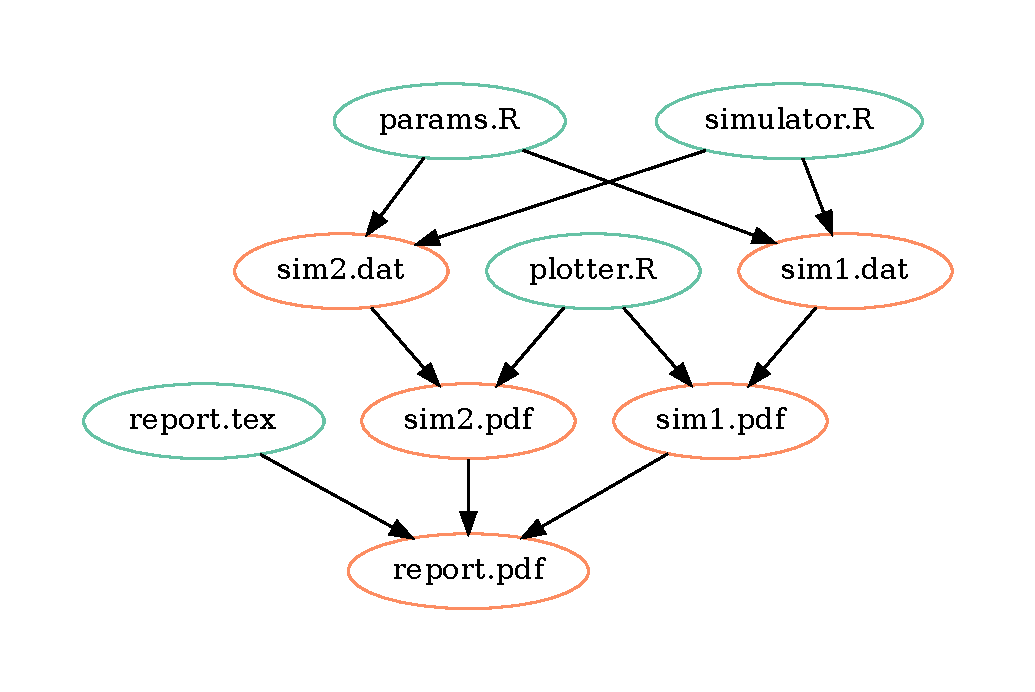
\includegraphics[width=12cm]{graph.pdf}

\end{frame}


\begin{frame}[fragile]
  \frametitle{Makefile conventions}

   - PHONY targets: denote actions; ignore filenames with same
     name. PHONY targets are always run.

\begin{verbatim}
.PHONY: all clean
all: report.pdf

clean:
        rm -f report.pdf report.log report.aux
        rm -f sim1.* sim2*

 |------------+---------------------------------------|
 | command    | action                                |
 |------------+---------------------------------------|
 | make       | check first rule                      |
 | make all   | rebuild everything                    |
 | make clean | remove files that can be rebuilt      |
 | touch file | update timestamp, preserving contents |
 |------------+---------------------------------------|
\end{verbatim}
\end{frame}



\begin{frame}[fragile]
  \frametitle{Makefile: next steps}

\begin{itemize}
\item variables
\item implicit rules
\item saving space:

\begin{verbatim}  
sim2.dat: params.R simulator.R
        Rscript simulator.R runif > sim2.dat

sim2.dat: simulator.R params.R
        Rscript $< runif > $@
\end{verbatim}
  
\item parallel processing \texttt{make -j8 jobs}
\end{itemize}

\end{frame}



\begin{frame}
  \frametitle{Further reading}
  \begin{itemize}
  \item Managing Projects with GNU Make \url{http://oreilly.com/catalog/make3/book/index.csp}

\item The GNU make manual \url{http://www.gnu.org/software/make/manual/make.html}

\item Tutorial (work in progress) \url{https://github.com/sje30/make-tutorial/blob/master/make-tut.pdf}
  \end{itemize}

\end{frame}

\begin{frame}
  \frametitle{2. Sweave: literate programming for R}

  \begin{enumerate}
  \item Sweave is the system for mixing \LaTeX\ and \R code in the same
    document.

  \item Used within \R often to create ``vignettes'' which can be
    dynamically run.

  \item Allows you to write reports where results (tables, graphs) are
    automatically generated by your \R code.
  \end{enumerate}
\end{frame}


\begin{frame}[fragile]
  \frametitle{Code chunks}

  By default we are in 'LaTeX mode', and we switch to code mode by using
  a code chunk.

  \verbatiminput{v.txt}
  
\end{frame}


\begin{frame}[fragile]
  \frametitle{What is markdown?}

  What is markdown?  A light-weight markup language for generating HTML.
\begin{verbatim}
### Example

Here is some *markup text* with **bold** and a
[link](http://www.rstudio.org).
Maths can be included $x^2 + y^2 = z^2$.
\end{verbatim}

  Useful also e.g. on github.
  

\end{frame}


\begin{frame}
  \frametitle{A full example}

  Estimate the value of $\pi$ using the dartboard method.

  \url{https://github.com/lgatto/spr/blob/master/estimate/estimatek.Rnw}

  shows how to include figures, tables, and caching feature.
\end{frame}


\begin{frame}
  \frametitle{What next?}

  Bookdown.org, vignettes, packages (https://devtools.r-lib.org/).
\end{frame}
\end{document}
